% Describe the test setup to verify that your problems from 1.3 have been solved.
% This can be done in different ways depending on focus of your problems.
% Some problems may purely objective, such as "improve the performance of X compared to Y".
% These are easy to evaluate since you simply need to compare the performance, and perhaps compare against a few more technologies that you have listed in Section 2 (related work).
% In other cases the problems may be very subjective, such as "Create a mobile app that can be used while driving, and which shows the most fuel efficient time to change gear".
% This problem will require a user-study in which several persons drive without the application, you calculate the fuel consumption, then they drive with the application and then you calculate the fuel consumption again.
% Then you collect the objective measurements (fuel consumption comparisons) and the subjective opinions from the users about whether the application was unobtrusive, usable, etc. (typically via a questionnaire).


TODO

\begin{figure}[h]
    \centering
    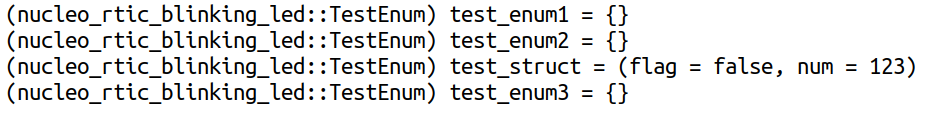
\includegraphics[width=1.0\textwidth]{lldb11.0-opt2-enum-edited.png}
    \label{fig:lldbenum}
\end{figure}


\begin{figure}[h]
    \centering
    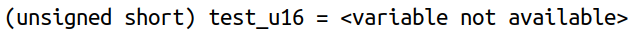
\includegraphics[width=1.0\textwidth]{lldb11.0-opt2-outofrange-edited.png}
    \label{fig:lldboutofrange}
\end{figure}

